%Author(s), Course variables
\newcommand{\titl}{Projektplan}
\newcommand{\courseno}{02121}
\newcommand{\course}{Indtroduktion til Softwareteknologi}
\newcommand{\lb}{\\}
%Basics
\documentclass[a4paper, danish]{article}
\usepackage[utf8]{inputenc}
\usepackage{babel}
\usepackage[moderate]{savetrees}
%Symbols and scientifics
\usepackage{amsmath, amsfonts, amssymb, bm}
\numberwithin{equation}{section}
\usepackage{physics}
\usepackage{mathtools}
\usepackage{siunitx}
\sisetup{
    per-mode = power ,
    round-mode = figures ,
    round-precision = 3 ,
    scientific-notation = false ,
    output-decimal-marker = {.} ,
    exponent-product = \times ,
    separate-uncertainty = true ,
    uncertainty-separator = \ ,
    range-phrase = - ,
    range-units =  single ,
    inter-unit-product = \ensuremath{{\cdot{}}} ,
    number-unit-product = \ ,
    multi-part-units = single ,
}

%Appendix, TOC and Bibliography
\usepackage{appendix}
\renewcommand\appendixtocname{Appendices}
\usepackage[nottoc]{tocbibind}
\setcounter{tocdepth}{2}
\usepackage{lastpage}

%Figures
\usepackage[svgnames]{xcolor} % Required to specify font color
\usepackage{float}
\usepackage{graphicx}
\usepackage{setspace}
\usepackage{subcaption}
\usepackage[format=plain,
    labelfont={bf,it,footnotesize},
    textfont={it,footnotesize}]{caption}
% \captionsetup[table]{name=Huskeord}
\captionsetup{font={stretch=0.9}}
\usepackage{wrapfig}
\usepackage[a4paper, centering, rmargin=2.5cm, tmargin=2.5cm, lmargin=2.5cm, bmargin=3.5cm]{geometry}
\usepackage{etoolbox}
\usepackage{verbatim}
\usepackage[space]{grffile}
\usepackage[final]{pdfpages}
\usepackage{array}
\usepackage{multirow}
\usepackage{dcolumn}
\usepackage{fontawesome}
\usepackage{tikz}
\usepackage{flowchart}
\usetikzlibrary{positioning, arrows}
\newcommand{\ttt}[1]{\texttt{#1}}
\newcommand{\F}{\mathtt{F}}
\newcommand{\T}{\mathtt{T}}
\usepackage{pgfgantt}
\usepackage{pdflscape}

\newcommand{\lorf}{\ensuremath{\lor\F}}
\newcommand{\lort}{\ensuremath{\lor\T}}
\newcommand{\landf}{\ensuremath{\land\F}}
\newcommand{\landt}{\ensuremath{\land\T}}
\newcommand{\tof}{\ensuremath{\to\!\F}}
\newcommand{\tot}{\ensuremath{\to\!\T}}
\newcommand{\lrf}{\ensuremath{\leftrightarrow\!\F}}
\newcommand{\lrt}{\ensuremath{\leftrightarrow\!\T}}
\newcommand{\negf}{\ensuremath{\neg\F}}
\newcommand{\negt}{\ensuremath{\neg\T}}
\newcommand{\allf}{\ensuremath{\forall\F}}
\newcommand{\allt}{\ensuremath{\forall\T}}
\newcommand{\exf}{\ensuremath{\exists\F}}
\newcommand{\ext}{\ensuremath{\exists\T}}

\newcommand{\first}[2]{\node (root) {\textcolor{red}{\scriptsize 1} \(#1\) : \texttt{#2}};}
\newcommand{\formula}[4]{\node (#1) [#2] {\textcolor{red}{\scriptsize #1} \(#3\) : \texttt{#4}};}
\newcommand{\branch}[2]{\path (#1) edge[-] (#2);}
\newcommand{\rbranch}[4]{\path (#3) edge[-] node [midway, right, blue] {\(#1\) på \(#2\)} (#4);}
\newcommand{\closed}[2]{\node (#1) [below = .1em of #2] {\(\times\)};}
\newcommand{\open}[2]{\node (#1) [below = .1em of #2] {\(\bigcirc\)};}
\newenvironment{tableau}{\begin{tikzpicture}[node distance = .5pt]}{\end{tikzpicture}}

%Header footer
\usepackage{fancyhdr}
\pagestyle{fancy}
\lhead{\titl \lb \courseno\ \course}
\chead{
\includegraphics[width=.05\textwidth]{DTU}}
\rhead{Aslan Behbahani, Yahya Alwan \\ Abinav Aleti, Rasmus Wiuff}
\cfoot{Side \thepage\, af \pageref*{LastPage}}
\renewcommand{\headrulewidth}{0.4pt}
\renewcommand{\footrulewidth}{0.4pt}
\setlength{\headheight}{36.75034pt}

%Text tools
\usepackage{listings}
\usepackage{parcolumns}
\usepackage[super]{nth}
\usepackage[normalem]{ulem}
\usepackage{import}
\usepackage{url}
\usepackage{lipsum}
\usepackage{microtype}
\usepackage[pdfencoding=auto, psdextra]{hyperref}
\hypersetup{
    colorlinks   = true, %Colours links instead of ugly boxes
    urlcolor     = blue, %Colour for external hyperlinks
    linkcolor    = blue, %Colour of internal links
    citecolor   = red %Colour of citations
}
\usepackage[capitalise]{cleveref}
% \crefname{table}{Huskeord}{Huskeord}
\usepackage{enumitem}
\newlist{arrowlist}{itemize}{1}
\setlist[arrowlist]{label={\(\rightarrow\)}}
\usepackage{booktabs}
\usepackage{todonotes}
\usepackage{silence}
\usepackage[square, longnamesfirst, numbers]{natbib}
\usepackage{empheq}
\usepackage{minted}
\setminted{fontsize=\small,
           linenos=true}
\usemintedstyle{tango}
\renewcommand{\listoflistingscaption}{Listings}
\newcommand{\im}[3]{\inputminted[linenos=true, python3=true, firstline=#2, lastline=#3]{python}{#1}}
\newcommand{\java}[3]{\inputminted[linenos=true, firstline=#2, lastline=#3]{java}{#1}}
\usepackage{tcolorbox}
\tcbuselibrary{skins,theorems}
\usepackage{pseudo}
\usepackage{tabularx}
\usepackage{tabto}
\TabPositions{1.5cm}
\pseudodefinestyle{fullwidth}{
    begin-tabular =
    \tabularx{\linewidth}[t]{@{}
        r
        >{\pseudosetup}
        X
        >{\leavevmode\small\color{blue}}
        p{0.5\linewidth}
        @{}},
    end-tabular =\endtabularx,
    setup-append = \RestorePseudoEq
}
\pseudoset{
    label=\small\arabic*,
    hd-space,
    ct-left = \hfill\texttt{*/},
    ct-right = \texttt{*/},
    ctfont = \texttt,
    fullwidth,
}
\newtcbtheorem[number within = section, crefname = {Algoritme}{algoritmer}]{algorithm}{Algoritme}{pseudo/tworuled, float}{alg}

%Definitions and new commands
\newcommand{\degr}{^{\circ}}
\newcommand{\me}{\mathrm{e}}
\newcommand*\mathinhead[2]{\texorpdfstring{\(\boldsymbol{#1}\)}{#2}}

%Title and sectioning
\def\Vhrulefill{\leavevmode\leaders\hrule height 0.7ex depth \dimexpr0.4pt-0.7ex\hfill\kern0pt}
\usepackage{titlesec}
\definecolor{DTUred}{cmyk}{0, .91, .72, .23}
\definecolor{FMNgrey}{cmyk}{.73,.43,.53,.38}
\newcolumntype{a}{>{\columncolor{gray}}c}
%Use letters insted of numbers in section numbering
% \renewcommand{\thesection}{\Alph{section}}
% \renewcommand{\thesubsection}{\Alph{subsection}}

\begin{document}

\titleformat{\section}[block]
{\normalfont\Large\scshape\filright\color{DTUred}}{\fbox{\thesection}}{1em}{}

\titleformat{\subsection}
{\titlerule
    \vspace{.8ex}%
    \normalfont\scshape\color{FMNgrey}}
{\thesubsection.}{.5em}{}

\title{\vspace{-4cm}
\includegraphics[width=.10\textwidth]{DTU}\lb\vspace{.5em}\Huge\scshape\color{DTUred} \titl\lb\vspace{-4mm}\rule{4cm}{0.5mm}\lb\Large{\courseno \ \course}}
\author{af \textbf{s224819} \ Aslan Dalhoff Behbahani, \ \textbf{s224739} \ Yahya Alwan,\\\textbf{s224786} \ Abinav Reddy Aleti \ og \ \textbf{s163977} \ Rasmus Wiuff \\ \textbf{Gruppe 16}}
\date{4. januar 2023}
\maketitle

\pagenumbering{arabic}

\thispagestyle{empty}

\section{Problemanalyse}
Projektet tager udgangspunkt i Model-View-Controller. Modelen deles udgør en klasse med en konstruktør for brættet og intern logik for placering og vending af brikker.
Vi benytter et heltals-array med tre stadier: 0 for et tomt felt, 1 for hvid brik og 2 for sort brik. En række metoder vil blive implementerede til at placere og vende brikker og kontrollere om et træk er lovligt. Reglerne afvikles også af \emph{bræt og brik} klassen. Reglerne og umiddelbare løsninger er beskrevet i \cref{tbl:logic}:
\begin{table}[H]
    \centering
    \caption{Regelsættets logiske implementering}\label{tbl:logic}
    \begin{tabular}{ll}
        \toprule
        Problem            & Løsning                                                                                 \\
        \midrule
        Startende spiller  & Spillere tildeles navne som tilfældigt tildeles farver. Hvid starter hver gang.         \\
        Startkonfiguration & Hvid farve får lov til at sætte to brikker. Sort placeres i de resterende midterfelter. \\
        Turbaseret spil    & Klasse med metoder der afgør om man skal melde pas,                                     \\
                           & om et træk skal gøres om samt om spillet er slut.                                       \\
        Afsluttet spil     & Metodekald til brætklassen, tæller vundet TN og afgør vinder.                           \\
        Uafgjort           & Spillet initialiseres igen med ny startende spiller.                                    \\
        Genstart           & Metodekald konstruere bræt-objektet igen og nye farver tildeles.                        \\
        \bottomrule
    \end{tabular}
\end{table}
Brugerfladen vil være et vindue indeholdende brættet med brikker, et tekstvindue der guider spillerne (hvis tur, skal der meldes pas, etc.), en pas knap og en genstart knap.
\section{Skitse over problemet}
I \cref{fig:logik} ses et flowchart der beskriver den interne logik, ud fra et spils gennemførsel. Diamandform viser brugervalg.
\begin{figure}[h]
    \centering
    \caption{Flowchart over programmets forløb}\label{fig:logik}
    \begin{tikzpicture}[font={\sf \small}]
        \node (start) at (0,0) [draw, terminal] {START};
        \node (construct) [right = .5 of start, draw, process] {Konstruer bræt};
        \node (view) [right = .5 of construct, draw, process] {Vis GUI};
        \node (colour) [right = .5 of view, draw, process] {Tildel farve};
        \node (initplace) [below right = .5 of colour, draw, decision] {Hvid: 2 brikker};
        \node (initplace2) [below left = .5 of initplace, draw, process] {Sort: 2 brikker};
        \node (logik1) [right = .5 of initplace, draw, process] {Ulovligt træk};
        % \node (pas) [left = .5 of logik1, draw, process] {}
    \end{tikzpicture}
\end{figure}
\section{Tilvalg af avancerede tilføjelser}
\cref{tbl:avanceret} viser mulige tilføjelser til den avancerede version i prioriteret rækkefølge.
\begin{table}[H]
    \centering
    \caption{Mulige avancerede tilvalg}\label{tbl:avanceret}
    \begin{tabular}{lllll}
        \toprule
        1: Brikker vendes automatisk & 3: Visning af mulige træk & 5: Spillernavne & 7: Gemme/Hente spil & 9: Visning af tid \\
        2: Visuelle effekter og lyd  & 4: Fullscreen             & 6: High-score   & 8: Valg af farver   & 10: Speed-Reversi \\
        \bottomrule
    \end{tabular}
\end{table}
\section{Delopgaver \& Tidsplan}
\cref{fig:gantt} viser den indledningsvise plan.
\begin{figure}[H]
    \centering
    \caption{Ganttdiagram over projektet}\label{fig:gantt}
    \begin{ganttchart}[
            expand chart = \textwidth,
            hgrid,
            vgrid,
            time slot format = isodate,
            % inline,
            % milestone inline label node/.append style={left=5mm},
            % milestone/.append style={xscale=.5},
        ]{2023-01-04}{2023-01-20}
        \gantttitlecalendar{month=shortname, day} \\
        \ganttgroup{BasicReversi}{2023-01-04}{2023-01-11} \\
        \ganttbar{Logisk model}{2023-01-04}{2023-01-06} \\
        \ganttbar{GUI implementering}{2023-01-04}{2023-01-10} \\
        \ganttbar{Test af BasicReversi}{2023-01-11}{2023-01-11} \\
        \ganttmilestone{BasicReversi færdig}{2023-01-11} \\
        \ganttgroup{AdvancedReversi}{2023-01-11}{2023-01-16} \\
        \ganttbar{Test af AdvancedReversi}{2023-01-17}{2023-01-18} \\
        \ganttmilestone{AdvancedReversi færdig}{2023-01-18} \\
        \ganttgroup{Rapportskriving}{2023-01-04}{2023-01-20} \\
        \ganttbar{Rapportafslutning}{2023-01-19}{2023-01-20} \\
        \ganttmilestone{Aflevering}{2023-01-20}
    \end{ganttchart}
\end{figure}
\end{document}